\chapter{实验步骤与实验结果}
\label{chap:implementation}

在这个部分中,我们讲述算法实现的具体步骤以及实验结果。
利用两组数据集,先生成满足条件的不完整信息网络,
然后使用距离学习算法学习距离。通过对比本文算法与kmeans算法的结果,
验证本文算法的可用性。

\section{实验环境}

CPU:Intel(R) Xeor(R) CPU E7420 @ 2.13GHz

内存:64G

操作系统:Microsoft Windows Server 2003 Enterprise x64 Edition

其中采用Python语言实现DSHRINK算法和局部信息网络的生成以及一些自动处理的脚本,
Python的版本是Python2.7。使用Matlab完成DCA算法,PCA分析以及画出结果图,
MATLAB版本为MATLAB version 7.8.0(R2009 a) 64位版 。

\section{社区挖掘的流程}

本文算法的整个流程如图\ref{fig:flow_chart}:

\begin{itemize}
    \item 首先选取合适的数据集用于实验;
    \item 由于数据集所得到的信息网络是完整的,需要对信息网络进行处理,使之满足满足本文关于局部信息网络的定义,
        也就是生成一个信息网络$G$,知道每一个节点的属性$X$,以及正语境限制$C$和负语境限制$D$;
    \item 基于$X, C, D$使用DCA学习一个距离度量,并计算节点对之间的距离;
    \item 基于距离用DSHRINK进行聚类。
\end{itemize}

\begin{figure}
    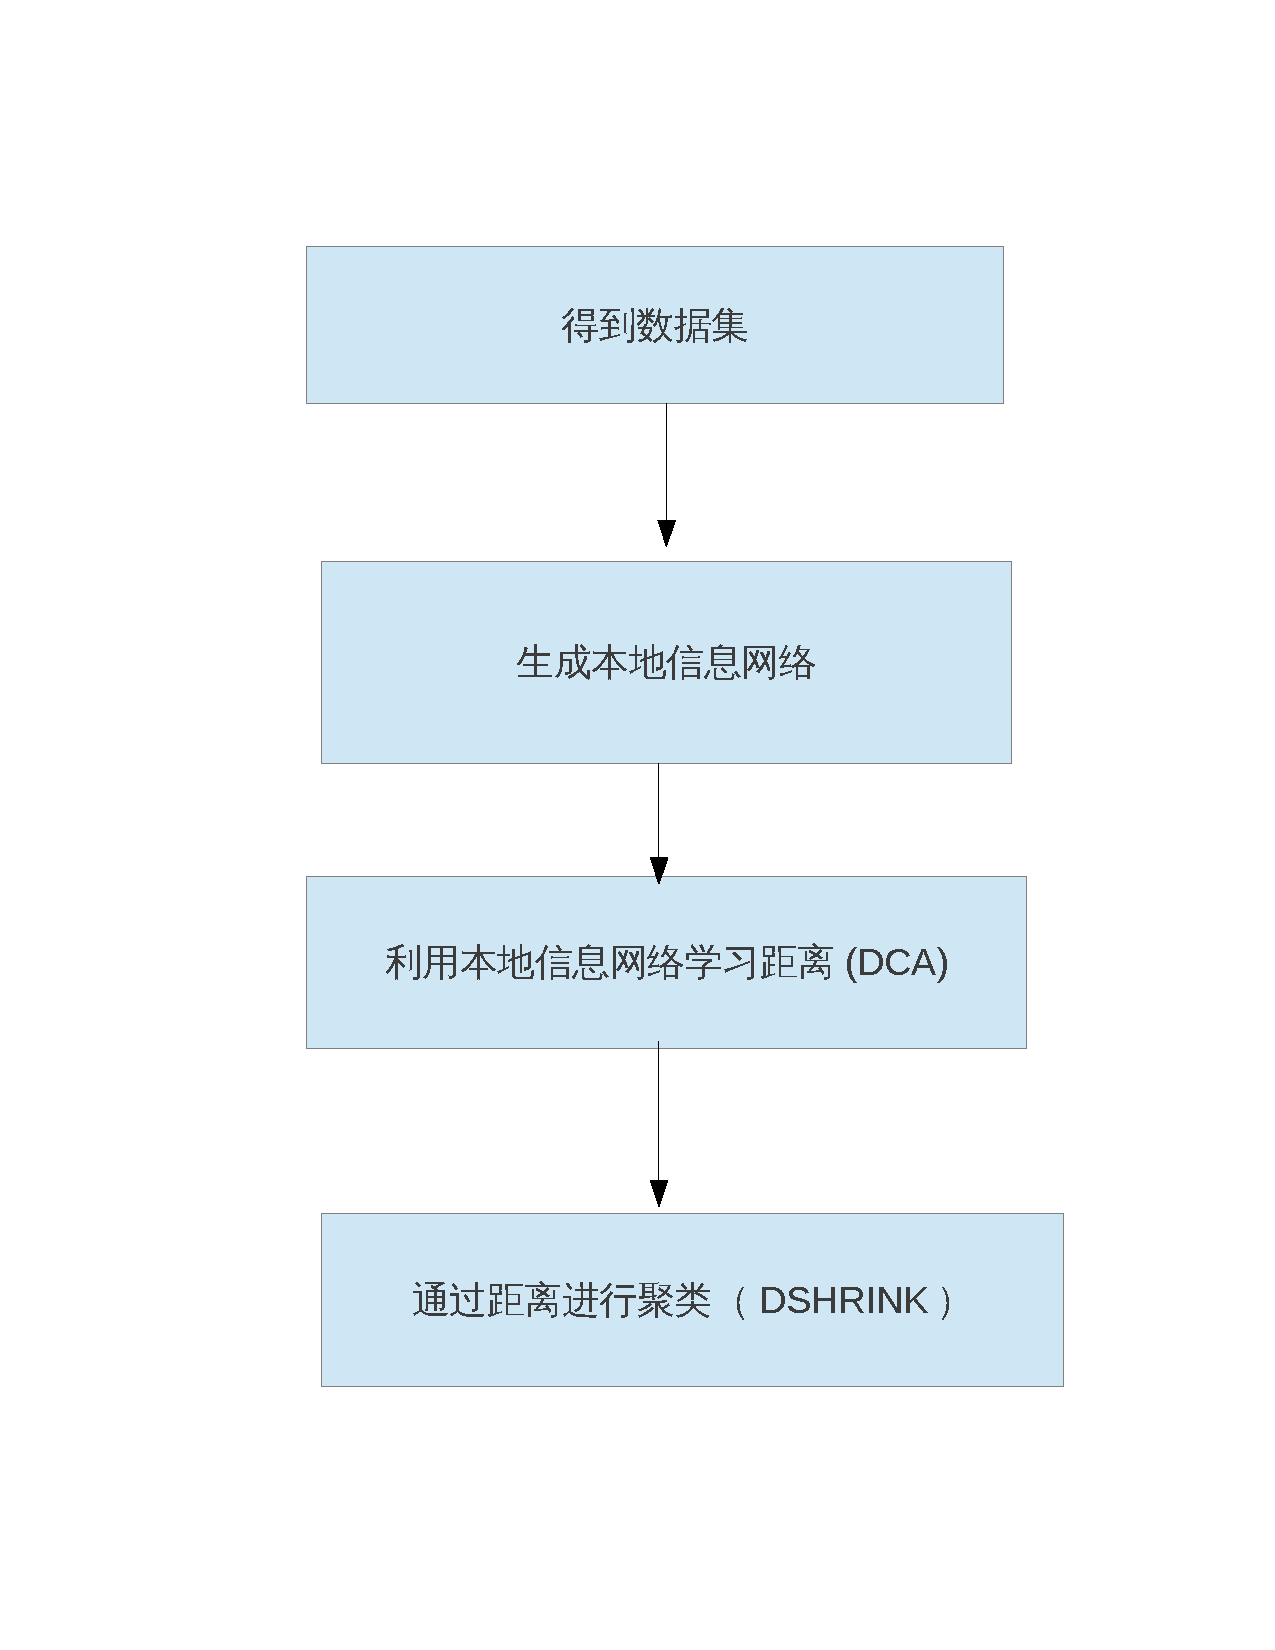
\includegraphics[width=1\textwidth]{flow_chart}
    \caption{社区挖掘的流程}
    \label{fig:flow_chart}
\end{figure}

在本章接下来的几节中,将对每个步骤做具体的介绍。

\section{数据集的选取}
\label{sec:imple:dataset}

本文实验使用两组数据集,均来自于
\href{http://www.blogcatalog.com/}{Blogcatalog},
Blogcatalog是一个博客社交网络, 它把人们与博客作者及博客作者与博客作者联系起来,
从Blogcatalog的数据中,我们可以得到由用户组成的社交网络。
经过处理,我们得到了一个由88784个节点组成的社交网络,每一个节点拥有5413个特征属性。
有60个类作为Ground Truth验证最后的聚类结果,其中每个节点属于60个类中的一个或多个。

由于节点数目过多,所以通过取样的方式生成两组数据集,对于每一组数据集取样的方法如下:
首先从60个中选取6个包含1000个左右节点的类,然后选取属于这6个类中的所有节点作为当前的数据集中的节点。
通过这种方式,得到了数据集Blogcatalog-a和Blogcatalog-b,分别包含5118和5209个节点。

在选定了节点之后,需要对节点的属性进行处理,因为对于每一个节点,大部分属性值都是0,
这样的属性不适合用欧氏距离或马氏距离作为节点之间的距离。所以采用主成分分析(Principle Component Analysis,PCA)对节点的属性进行降唯,
最终选定了50个属性作为节点的属性。在使用PCA分析之前,必须对节点的属性正规化(Normalize)。

最终数据集的特征总结见表\ref{tab:datasetsummary}。

\begin{table}[!hpb]
  \centering
  \caption{实验采用数据集总结}
  \label{tab:datasetsummary}
  \begin{tabular}{rrrrr} \toprule
    数据集 & 节点数 & 边数  & 属性数 & 类个数\\ \midrule
    Blogcatalog-a & 5118 & 22863 & 50 & 6 \\
    Blogcatalog-b & 5118 & 25761  & 50 & 6 \\ \bottomrule
  \end{tabular}
\end{table}


\section{生成局部信息网络}

为了使用DCA距离学习算法,必须生成满足条件的不完全信息网络。
也就是说,必须要生成正语境限制和负语境限制。
本文生成正语境限制和负语境限制的方法如下:

为了生成正语境限制,必须找到相似集列表$C$,
需要在整个信息网络中取样一定数目的节点来生成$C$,
利用局部信息网络的特点,可以通过生成一定数量的特定大小的局部信息网络,
利用这些局部信息网络中的节点来生成$C$。定义局部信息网络的个数为regionNum,
局部信息网络的大小为regionSize。我们首先对节点按照与节点想关联的边的个数进行排序,
然后依次挑选一个节点作为一个局部信息网络的起始节点。对于第一个局部信息网络,
拥有边最多的节点被选中作为其实节点,然后利用宽度优先搜索(Broad First Search, BFS)添加节点到当前的局部信息网络,
直到regionSize个节点被添加。同样地,从排序的节点的列表中挑选边最多的未被访问的节点作为第二个局部信息网络的起始节点,
然后使用BFS添加节点,
依次类推直到生成regionNum个局部信息网络。利用这regionNum个局部信息网络所包含的节点来生成正语境限制。
对于任意两个节点,如果它们属于同样的类,那么它们就是相似的节点对,应该属于同样的相似集。
如果相似集$C_i$中的某个节点与相似集$C_j$相似,那么把$C_i$和$C_j$合并成一个相似集。

生成负语境限制的方法相对简单,只需要随机选取regionNum乘regionSize个节点用于生成负语境限制。
如果相似集$C_i$中的某个节点与相似集$C_j$不相似,那么$j \in D_i$且$i \in D_j$。

在已知了相似节点对列表S和不相似节点对列表D之后,生成正负语境限制的详细过程见\ref{code:constraint},
S的格式$[(u_1, v_1), (u_2, v_2), ...]$其中每一项对应的两个节点都相似,
D的格式$[(u_1, v_1), (u_2, v_2), ...]$其中每一项对应的两个节点都不相似,
输出chunks, 正语境限制和neglinks, 负语境限制。
首先初始化chunks, 每一个节点都没有分配chunk,对应的chunkId是-1。
然后遍历S,生成正语境限制。对于S中任意节点对u,v:
\begin{inparaenum}[a)]
    \item 如果它们都没有分配chunk, 把他们分配到一个新的chunk里;
    \item 如果只是其中一个没有分配chunk,把它分配到另一个的chunk;
    \item 如果两个都分配了chunk,那么合并这两个chunk。
\end{inparaenum}
然后开始生成负语境限制,首先初始化为neglinks为全0矩阵,
也就是说对于任意两个chunks来说,它们不相似的程度为0。
然后遍历D更新neglinks,对于D中的任意两个节点u,v,
如果他们属于不同的已经分配的chunks,那么对应的neglinks加1。

\section{结果好坏的评价标准}

为了评价本文提出算法的有效性,通过对比本文提出的算法和kmeans在Blogcatalog和
Blogcatalog-b上结果的好坏来判定。基于Ground Truth中包含的类的信息,我们使用聚类的纯度(Purity)来作为结果好坏的标准。
纯度的定义如下:

对于每一个聚类,在这个聚类中拥有最多节点个数的类作为这个聚类的标签,
属于这个标签的节点的个数是聚类的标签计数,
纯度等于所有聚类的标签计数和除以所有的节点个数。
数学表达为:

\begin{equation}
\label{equa:purity}
Purity = \frac{1}{n} \sum_{i=1}^k \operatorname{max}_j |C_i \bigcap l_j|
\end{equation}

其中$\{C_1, ..., C_k\}$是所有的聚类,$\{l_1, ..., l_j\}$是所有的类。
根据定义可以知道,纯度越高,聚类的效果越好。

计算纯度的代码见\ref{code:purity}。

\begin{lstlisting}[language={python}, caption={计算聚类的纯度}, label=code:purity]

# 根据划分的聚类计算纯度
# 输入clusters: 得到的一个个聚类
# 输入NODE_NUM: 节点的个数
# 输入usercategory: 用于验证
def get_purity(clusters, NODE_NUM, usercategory):
    purity_sum = 0 # 所有类的标签计数的和,初始化为0

    for cluster in clusters:
        purity_sum += get_max_pi(cluster, usercategory)

    return float(purity_sum) / NUM_NODES #返回标签计数的和除以节点个数作为纯度

# 得到一个聚类的标签计数
# 输入cluster: 聚类,节点列表[c_1, c_2...] 
# 输入usercategory: 用于验证
def get_max_pi(cluster, usercategory):
    category_count = [0] * NUM_CATEGORY #需要统计每一个类所拥有的节点个数,初始化都为0
    
    # 如果有一个节点属于某一个类,那么这个类的节点个数加1
    for node in cluster:
        for category in range(NUM_CATEGORY):
            if usercategory[node][category] == '1':
                category_count[category] += 1

    return max(category_count) #返回所有类中最大的节点个数作为这个聚类的标签计数

\end{lstlisting}


\section{自动化实验}

在完成本文实验的过程中,需要观察DSHRINK和Kmeans在两组数据集下的结果。
对于每一个数据集,需要考察在不同的局部信息网络大小和不同的局部信息网络个数下的纯度,
而且,对于每一种情况都需要重复实验5次去平均值作为实验结果。
这需要进行大量的实验,因此需要一种自动化完成实验的方法。
为此,我们实现了一个自动化的脚本,
运行一次这个脚本能够完成整个实验的过程。

自动化脚本的实现代码见\ref{code:auto}, 分别两组数据集Blogcatalog-a和Blogcatalog-b进行实验,对于每个数据集,
分别研究在不同的局部信息网络大小和不同的局部信息网络个数下面社区挖掘的结果,同时对于每一种情况,重复实验5次,
取平均值作为实验结果。在每次实验时,首先生成正负语境限制,然后利用DCA算法进行距离度量学习,
然后调用DSHRINK算法进行聚类,最后计算出聚类的纯度。
由于自动化脚本采用Python语言实现,
而整个实验过程除了DCA算法之外都采用Python语言实现,
为了实现自动化的过程,必须能够在Python语言中调用matlab的脚本。
我们经过研究,可以直接通过代码\ref{code:call}实现。

\begin{lstlisting}[language={python}, caption={计算聚类的纯度}, label=code:call]

# 引入模块用于执行系统命令
import os

# 根据数据集的不同,组合出不同的命令,用于调用
pre_command = r"""matlab -nodisplay -nosplash -nodesktop -wait -r "run('"""
post_command = r"""');exit;" """
script_name = "%s\dca_distance.m" % data_set
command = pre_command + script_name + post_command

# 调用系统的命令
os.system(command)
\end{lstlisting}

\section{实验结果}
\label{sec:results}
对于数据集Blogcatalog-a和Blogcatalog-b,
分别观察在不同的局部信息网络大小(一个局部信息网络中的节点个数)
和不同的局部信息网络的个数情况下的实验结果。
由于算法具有一定的随机性,对于每一种不同的情况,
重复实验5次,取平均值作为实验结果。

\subsection{不同的局部信息网络的大小}
\label{sec:results_node_max}

在Blogcatalog-a和Blogcatalog-b做社区挖掘所得到的纯度随局部信息网络大小不同的变化如图\ref{fig:node_max:a}和图\ref{fig:node_max:b}。
此时选取的信息网络的个数为10。从实验结果可以看出,DSHRINK总是能比kmeans有更好的纯度,
同时总体的趋势是随着局部信息网络大小的增加,纯度变高。

\begin{figure}
    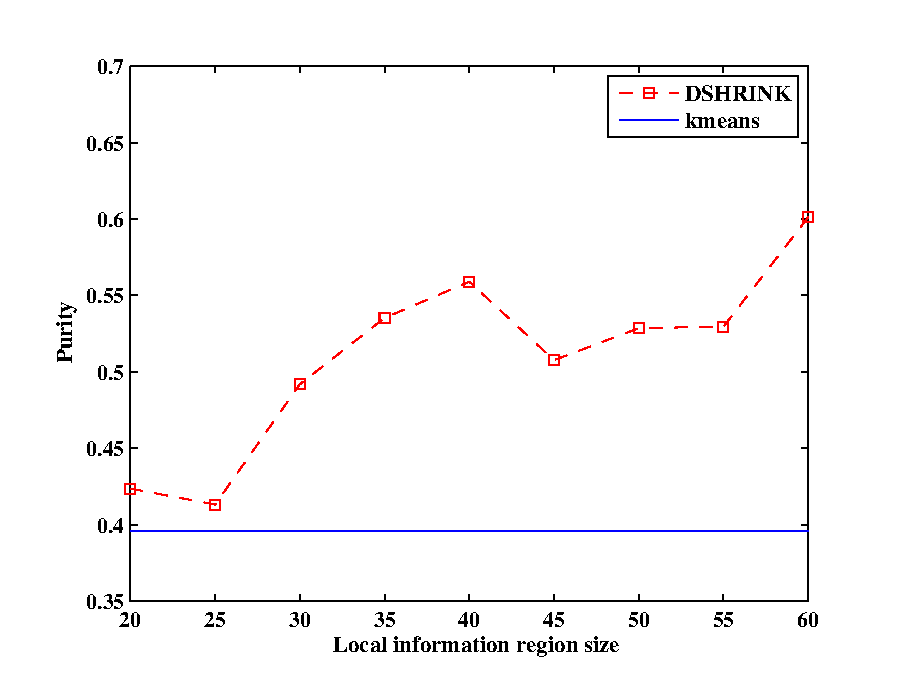
\includegraphics[width=1\textwidth]{chap2/blogcatalog_node_max}
    \caption{Blogcatalog-a在不同局部信息网络大小下的纯度}
    \label{fig:node_max:a}
\end{figure}

\begin{figure}
    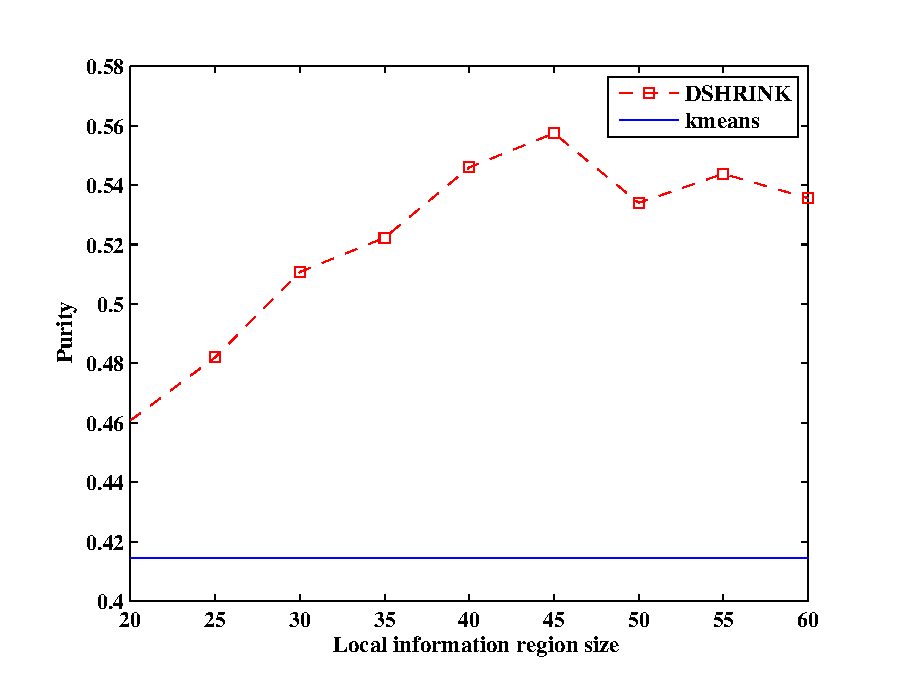
\includegraphics[width=1\textwidth]{chap2/blogcatalog_b_node_max}
    \caption{Blogcatalog-b在不同局部信息网络大小下的纯度}
    \label{fig:node_max:b}
\end{figure}

\subsection{不同的局部信息网络个数}
\label{sec:results_region_num}

在Blogcatalog-a和Blogcatalog-b做社区挖掘所得到的纯度随局部信息网络大小不同的变化如图\ref{fig:region_num:a}和图\ref{fig:region_num:b}。
此时选取的信息网络的大小为50。从实验结果可以看出,DSHRINK总是能比kmeans有更好的纯度,
同时总体的趋势是随着局部信息网络大小的增加,纯度变高。

\begin{figure}
    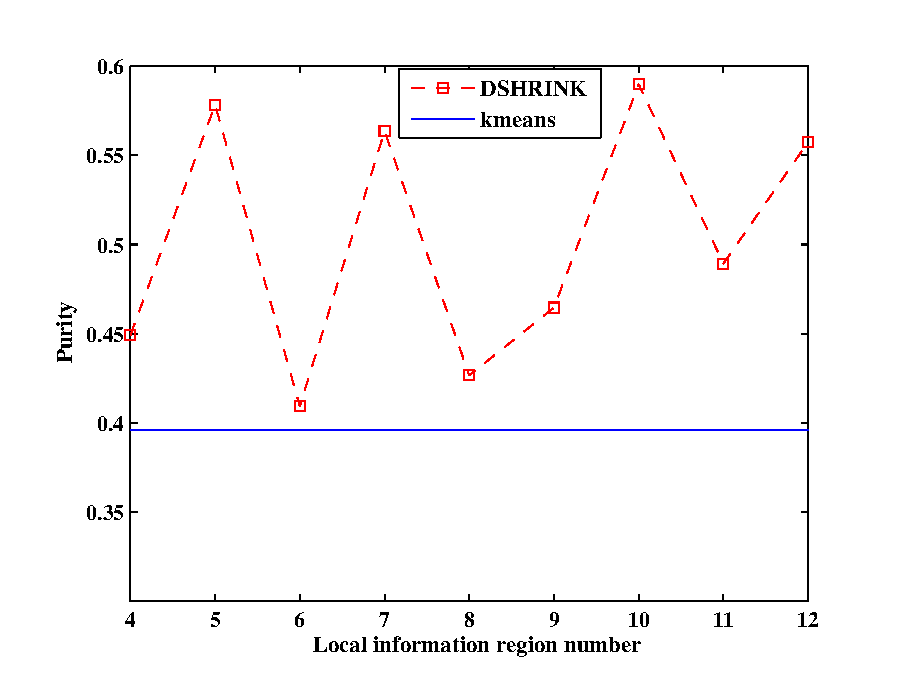
\includegraphics[width=1\textwidth]{chap2/blogcatalog_region_num}
    \caption{Blogcatalog-a在不同局部信息网络个数下的纯度}
    \label{fig:region_num:a}
\end{figure}

\begin{figure}
    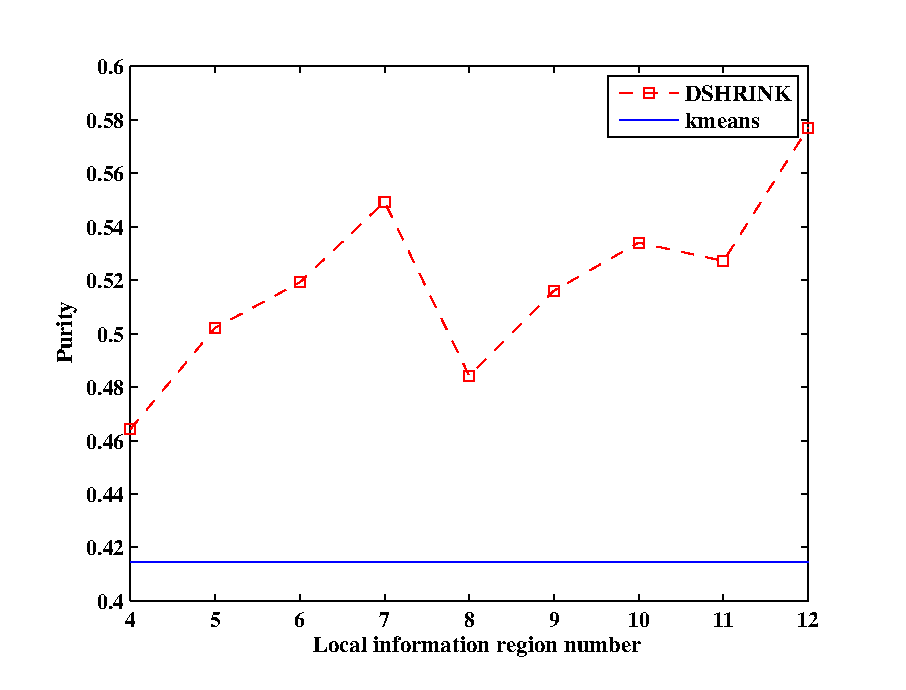
\includegraphics[width=1\textwidth]{chap2/blogcatalog_b_region_num}
    \caption{Blogcatalog-b在不同局部信息网络个数下的纯度}
    \label{fig:region_num:b}
\end{figure}

\subsection{实验结果分析}

DSHRINK相对于kmeans有更高的纯度是因为kmeans只是单纯地根据节点之间的欧式距离进行聚类,
而DSHRINK根据已知的信息在欧式距离的基础上进行了一定的调整,
这个距离能够保证相似的节点之间的距离更近,不相似的节点之间的距离更远。
基于这个距离对节点进行聚类,
能够达到更好的聚类效果。
而且,局部信息网络的个数越多或者局部信息网路的大小越大,知道的信息越多,
使用本文提到的算法进行聚类的纯度越高。

同时,DSHRINK聚类能够根据模块性准则自动地得到一个合适的聚类个数,而对于kmeans来说,
必须要先确定聚类的个数K才能聚类。对于实际的问题来说,聚类的个数是未知的,
此时如果要使用kmeans算法的,就必须尝试各种不同的k来确定达到一个比较好的聚类效果。
确定k的过程需要进行大量的实验,是一个十分耗时的过程。从这一点上,
本文算法具有相当大的优势。另外,从实验的过程中我们发现,
最终结果的好坏和选取的$\epsilon$没有关系,但是更大的$\epsilon$能够导致在每次迭代的过程中,有更多的节点被
合并到一个当地社区,因此能够减少迭代的次数,加快整个实验的运行。

\section{本章小节}

在本章中,我们详细阐述了实现本文算法实现时的实验环境与实验的各个步骤。
同时,通过对比本文算法和kmeans算法在不同的数据集和不同局部信息网络下的实验结果,
得出本文算法能够比kmeans算法在信息缺失的信息网络中具有更好地效果,
具有很好的实用性。
